\documentclass[a4paper,12pt]{article}
\usepackage[utf8]{inputenc}
\usepackage{amssymb,amsmath,amsfonts}
\usepackage{graphicx,graphics}
\usepackage{lipsum}
\usepackage{multicol}
\usepackage{mathtools}
\usepackage{pstricks}
%\usepackage{pstricks-add}
%\usepackage{pst-func}
\usepackage{pst-plot}
\usepackage{pst-xkey}
\usepackage{anysize}
\marginsize{2cm}{2cm}{1.5cm}{2cm} %izq,der,arr,abj%
%\stackrel{\text{compacidad}}{=}

\newcommand{\NN}{\mathbb{N}}
\newcommand{\RR}{\mathbb{R}}
\newcommand{\QQ}{\mathbb{Q}}
\newcommand{\ZZ}{\mathbb{Z}}
\newcommand{\calA}{\mathcal{A}}
\newcommand{\calB}{\mathcal{B}}
\newcommand{\calC}{\mathcal{C}}
\newcommand{\Ra}{\Longrightarrow}
\newcommand{\Le}{\Leftarrow}
\newcommand{\longLe}{\Longleftarrow}
\newcommand{\gpar}[1]{\left({#1}\right)}
\newcommand{\sii}{\Longleftrightarrow}
\newcommand{\ds}{\displaystyle}
\newcommand{\fail}{\Rightarrow\Leftarrow}
%\newcommand{\vs}{\vspace}
\newcommand{\hs}{\hspace}
\newcommand{\dd}{\dfrac}
\newrgbcolor{asd1}{0.65 0.498 0.274}
\newrgbcolor{gray}{0.7 0.7 0.7}
\newrgbcolor{zzttqq}{0.6 0.2 0}

\setlength{\parskip}{10pt}


\begin{document}
\begingroup
\setlength{\parindent}{0pt}

\begin{center}
	\huge $$\sqrt{\scalebox{2.1}{$\tau$}}$$
	\Large Trøndelagkonkurranse 2026 - Level I\\[2pt] First round - 26.09\\
	1st part
\end{center}
\vspace{1cm}

{\bf Choose and solve only one of the following problems:}

\vspace{.7cm}
{\bf Problem 1}

Nils and Bianca are studying a particular type of fly, the {\it rubrum diptera}. These flies are born blue, and 24 hours after being born, they turn red. Then, 24 hours after they have turned red, if they have eaten the necessary amount of food, they give birth to a blue fly.

As long as they keep eating, the dipteras keep reproducing every 24 hours.

Assuming the dipteras eat the necessary amount of food constantly once they are born, determine if the size of a swarm from one fly can eventually reach a size of exactly $N=2026$. 

\vspace{.7cm}
{\bf Problem 2}

Bianca wrote the following numbers on the whiteboard
$$A,B,C,D,E,F$$
such that any of those values is either $0,1,2,3,\ldots$ up to 9. Nils noticed that he could form three pairs of numbers; for example, $(A,B),(C,D)$ and $(E,F)$, such that the product of each pair has 1 as the last digit; for example, the last digit of $3\cdot4$ is 2.

If all the pairs are different, determine the possible values of $A+B+C+D+E+F$.

(The pairs (1,2) and (2,1) are the same, but (2,3) and (3,3) are not.)


\newpage %-----------------------------------


\begin{center}
	\huge $$\sqrt{\scalebox{2.1}{$\tau$}}$$
	\Large Trøndelagkonkurranse 2026 - Level I\\[2pt] First round - 26.09\\
	2nd part
\end{center}
\vspace{1cm}

Bianca proposes the following problem to Nils, she constructs a big triangular array of numbers as shown below 

\begin{center}
	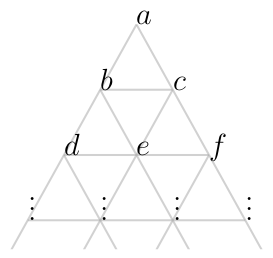
\includegraphics[scale=0.5]{im3.png}
\end{center}

such that the possible values of $a,b,c,$ and so on are $-1,0$ and 1. She first chooses one value for $a$, and then randomly assigns values making sure that no two adjacent values are equal.

{\bf Task 1:} If the bottom of the array has 6 numbers, show that the sum of all the values in the array is independent of the choice of $a$.

{\bf Task 2:} If the bottom of the array has 2025 numbers, show that the sum of all the values in the array is independent of the choice of $a$.

Nils, would also like to give Bianca a similar problem, either using arrays of numbers or sums of integers or anything interesting he can think of.

{\bf Task 3:} Help Nils create a nice problem he can give to Bianca.


\endgroup
\end{document}










